\documentclass{prova}

\usepackage{amsmath}
\usepackage{amsfonts}
\usepackage{gensymb}

\setlength{\textheight}{25cm}

\renewcommand{\sin}{\,\mbox{sen}\,}
\newcommand{\ds}{\displaystyle}

\professor{Prof.\@ Adriano Barbosa}
\disciplina{C\'alculo Diferencial e Integral III}
\avaliacao{PS}
\curso{Engenharia Mecânica}
\data{01/06/2021}

\begin{document}
	\cabecalho{5}  % o numero 5 indica a qnt de quadros na tabela de nota

    \textbf{Todas as respostas devem ser justificadas.}

    \textbf{Resolva apenas a avalia\c{c}\~ao referente a sua menor nota.}
    \vspace{0.5cm}

    {\bf Avalia\c{c}\~ao P1:}
    \begin{questionario}
        \q{Determine se as afirmações são verdadeiras ou falsas e justifique sua resposta:}
            \begin{questionario}
                \qq{Seja $f(x,y) = \ds\frac{x^3y}{x^6+y^2}$. Tomando o caminho $y=x^3$:}
                    \[y=x^3: f(x,x^3) = \frac{x^3x^3}{x^6+(x^3)^2} = \frac{x^6}{2x^6} = \frac{1}{2}.\]
                    Portanto, $\ds\lim_{(x,y)\rightarrow (0,0)} f(x,y) = \frac{1}{2}$.
                \qq{Se o gráfico de $f(x,y)$ é um plano, então as derivadas
                    parciais de primeira ordem de $f$ são nulas.}
            \end{questionario}
        \q{Num retângulo o comprimento e a largura são medidos como 30 cm e 24 cm,
            respectivamente, com um erro de 0,1 cm em cada medida. Use a aproximação linear
            da área para estimar o erro máximo no cálculo da área, onde o erro é dado por $|$área
            medida - área aproximada$|$.}
        \q{Os quatro tipos de sangue são determinados pelos alelos A, B e O. A
            proporção de indivíduos numa população que carregam dois alelos
            diferentes é $P = 2ab+2ac+2cb$, onde $a$, $b$ e $c$ são as
            proporções de $A$, $B$ e $O$ na população. Sabendo que $a+b+c=1$,
            mostre que $P$ é no máximo $\frac{2}{3}$.}
        \q{A profundidade de um lago é dada em função das coordenadas no plano de sua
            superfície como $z = 200-0,02x^2-0,001y^3$. Um pescador está no ponto $(40, 30)$
            e se move na direção de uma boia que está no ponto $(0,0)$. A profundidade do lago
            está aumentando ou diminuindo no momento em que ele inicia o trajeto?}
    \end{questionario}

    \vspace{1cm}

    \pagebreak
    {\bf Avalia\c{c}\~ao P2:}
	\begin{questionario}
        \q{Calcule a área da região limitada pela rosa $r=\cos(2\theta)$.}
            \begin{figure}[!h]
                \centering
                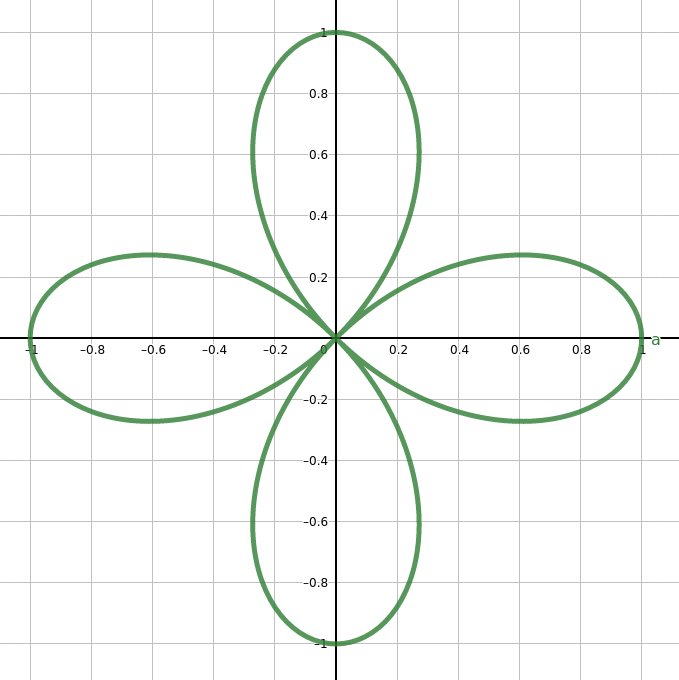
\includegraphics[width=0.3\textwidth]{rosa.png}
            \end{figure}
        \q{Calcule o volume do toro $\rho=\sin(\phi)$.}
            \begin{figure}[!h]
                \centering
                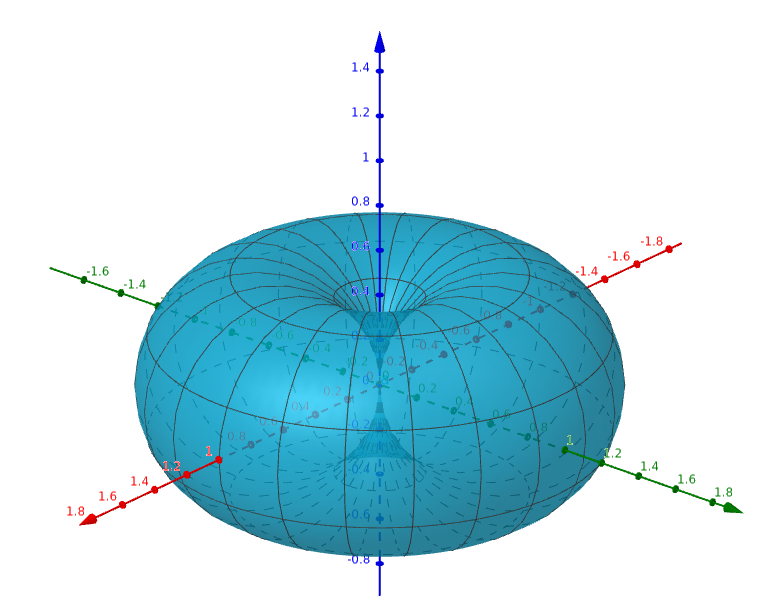
\includegraphics[width=0.5\textwidth]{toro.png}
            \end{figure}

            Use $\ds\int \sin^4(x)\ dx = \frac{3}{8}x - \frac{1}{4}\sin(2x) +
            \frac{1}{32}\sin(4x) + C$, se necessário.
        \q{Calcule o trabalho realizado pelo campo $\ds F(x,y) =
            \left(\frac{x}{x^2+y^2}, \frac{y}{x^2+y^2}\right)$, ao mover uma
            partícula ao longo do círculo unitário de centro na origem no
            sentido anti-horário.}
        \q{Sejam $F(x,y) = (x^3+y, 3x-2y)$ e $C$ é a borda de um triângulo 
            de área 3 e está orientada positivamente. Calcule
            $\ds\int_C F\cdot\ dr$.}
	\end{questionario}
\end{document}
